%
% Background
%
\chapter{Background} \label{sec:background}
We will first discuss relevant background work regarding reinforcement learning, continual learning, and competitive Pokémon.

\section{Reinforcement Learning} \label{sec:rl}
Reinforcement learning (RL) is a machine learning paradigm in which an agent learns to make sequential decisions by interacting with an environment~\cite{sutton2018rl,sutton1992rl,sutton1999rl}.
Unlike supervised learning, where training data consists of labeled pairs, reinforcement learning relies on evaluative feedback in the form of rewards, with the objective being to learn a policy that maximizes the expected cumulative reward over time~\cite{sutton2018rl,sutton1999rl,wang2024drl}.

A reinforcement learning problem is typically formulated as a Markov decision process (MDP), defined by the tuple $(\mathcal{S}, \mathcal{A}, \mathcal{P}, \mathcal{R}, \gamma)$~\cite{khetarpal2022crl,puterman1990mdp}:
\begin{itemize}
    \item $\mathcal{S}$: The set of states representing possible configurations of the environment.
    \item $\mathcal{A}$: The set of possible actions available to the agent.
    \item $\mathcal{P}(s^\prime | s, a)$: The transition probability function that describes the probability of transitioning to state $s^\prime$ after selecting action $a$ in state $s$.
    \item $\mathcal{R}(s, a)$: The immediate reward obtained after performing action $a$ in state $s$.
    \item $\gamma \in [0, 1)$: The discount factor, balancing the importance of immediate and future rewards.
\end{itemize}
At each time step $t$, the agent observes a state $s_t$, selects an action $a_t$ according to a policy $\pi(a|s)$, receives a reward $r_t$, and transitions to a new state $s_{t+1}$~\cite{sutton2018rl}.
The Markov assumption states that the next state and reward depend only on the current state and action, allowing the decision process to be represented without requiring the complete interaction history~\cite{puterman1990mdp}.
The objective of the agent is to learn an optimal policy $\pi^*$ that maximizes the expected (discounted) return~\cite{sutton2018rl,khetarpal2022crl}:
\begin{equation}
    G_t = \sum_{k=0}^{\infty}\gamma^k r_{t+k+1}
\end{equation}

In practice it is quite uncommon for an agent to be able to directly observe the full underlying state $s_t$.
The specific information that an agent receives or perceives through its sensors is called an \textit{observation}, denoted by $o_t \in \mathcal{O} \subseteq \mathcal{S}$~\cite{sutton2018rl,kaelbling1998pomdp}.
Observations generally lack the full information needed to accurately determine the true state, leading to a partially observable Markov decision process (POMDP)~\cite{kaelbling1998pomdp}.

The expected return when following policy $\pi$ from state $s$ is given by the state-value function $V^\pi(s)$~\cite{sutton2018rl,stefano2024marl}:
\begin{equation}
    V^\pi(s) =  \mathbb{E}_\pi[G_t \mid s_t=s] = \sum_{a \in \mathcal{A}} \pi(a|s) \left[ \mathcal{R}(s, a) + \gamma \sum_{s^\prime \in \mathcal{S}} \mathcal{P}(s^\prime | s, a) V^\pi(s^\prime) \right]
\end{equation}
Similarly, the expected return when following policy $\pi$ after taking action $a$ in state $s$ is given by the action-value function $Q^\pi(s, a)$, typically called the \textit{Q-value} of a state-action pair $(s, a)$~\cite{sutton2018rl,stefano2024marl}:
\begin{equation}
    Q^\pi(s, a) = \mathbb{E}_\pi[G_t \mid s_t=s, a_t=a] = \mathcal{R}(s, a) + \gamma \sum_{s^\prime \in \mathcal{S}} \mathcal{P}(s^\prime | s, a) V^\pi(s^\prime)
\end{equation}

One of the main challenges that arises in reinforcement learning is the inherent trade-off between exploration and exploitation.
The agent has to exploit its learned knowledge to obtain a lot of reward, but to learn said knowledge and make better decisions in the future it must explore other actions as well.
Neither exploration nor exploitation can be exclusively pursued without failing at finding the optimal policy~\cite{sutton1999rl}.

Traditional reinforcement learning algorithms learn value functions from which policies are derived, often through a greedy selection strategy.
A common way to balance exploration and exploitation in such algorithms is through the $\epsilon$-greedy selection strategy, with the parameter $\epsilon$ denoting the probability of choosing a random action (exploration), and $1 - \epsilon$ denoting the probability of greedily choosing the best action (exploitation)~\cite{sutton2018rl,sutton1999rl,stefano2024marl}:
\begin{equation}
    \pi(s) = 
    \begin{cases}
        \text{random } a \in \mathcal{A} & \text{with probability } \epsilon \\
        \argmax_a Q^\pi(s, a) & \text{with probability } 1 - \epsilon
    \end{cases}
\end{equation}

An agent learning directly from the actions it takes while following its current policy is learning \textit{on-policy}.
Conversely, an agent learning a different policy than it currently uses to navigate the environment is learning \textit{off-policy}~\cite{sutton2018rl}.
On-policy learning is traditionally more stable, but less sample efficient as it only learns from each experience once before discarding it~\cite{sutton2018rl,wang2024drl}.
Off-policy learning is more efficient as it can keep a replay buffer of past experiences to keep learning from, but it can be less stable and prone to divergence if the data becomes too outdated~\cite{sutton2018rl,hasselt2018deadlytriad,lin1992replaybuffer}.

\subsection{Deep Reinforcement Learning} \label{sec:rl:deeprl}
As the complexity of the environment increases, keeping explicit track of the policy or value function becomes computationally intractable~\cite{sutton2018rl,wang2024drl}.
To overcome this limitation, deep reinforcement learning (DRL) agents use function approximators like artificial neural networks as value functions or policies~\cite{wang2024drl}.
An established example of DRL is deep Q-networks, using a deep neural network to approximate Q-values for all actions in a given state simultaneously~\cite{mnih2015dqn}.

In general, DRL agents do not learn a direct mapping from states to actions, but instead learn a mapping from states to a probability distribution of actions, $\pi: \mathcal{S}, \mathcal{A} \rightarrow \mathbb{R}$~\cite{sutton2018rl,wang2024drl}.
Following such a policy helps balance between exploration and exploitation, as the agent now sometimes selects sub-optimal actions that explore new directions, albeit at a lower probability.
In the context of artificial neural networks, the final layer of the network often predicts raw, unnormalized numerical `scores' for each action, called \textit{logits}.
These logits can then be converted to a probability distribution of actions using the softmax function~\cite{sutton2018rl,bridle1990softmax}:
\begin{equation}
    \text{softmax}(x_i) = \frac{e^{x_i}}{\sum_j e^{x_j}}
\end{equation}

\begin{figure}[ht]
    \centering
    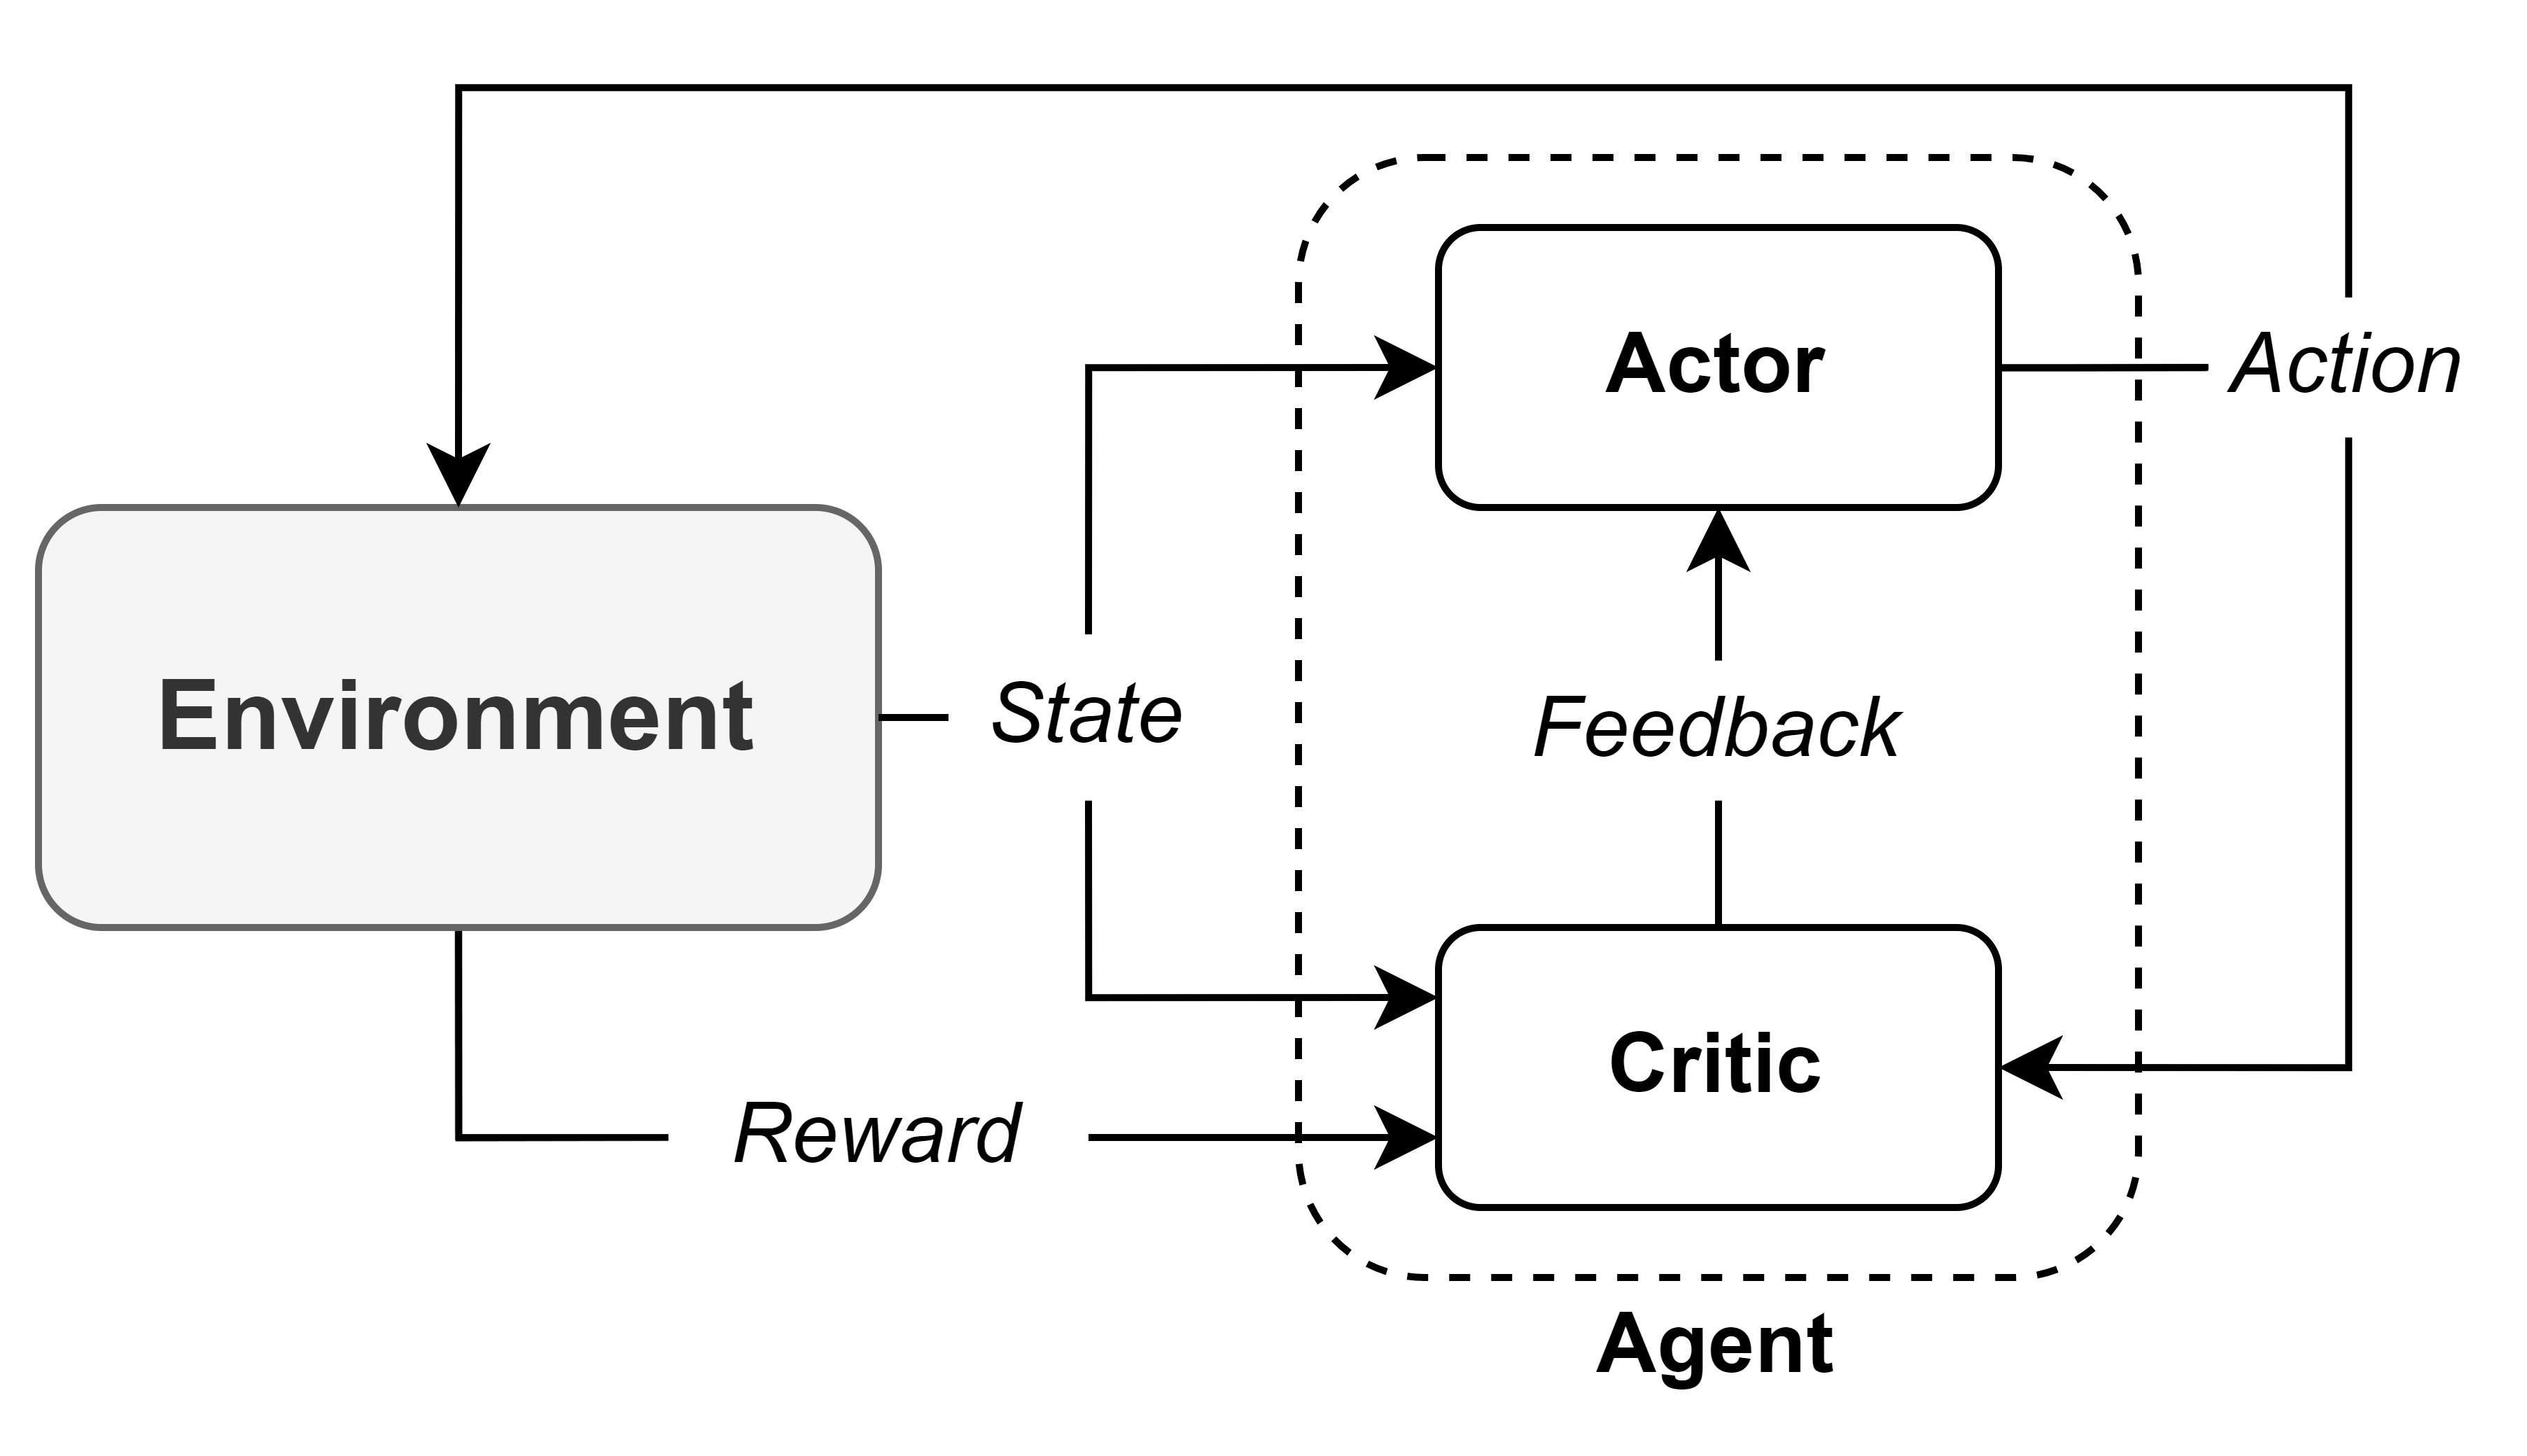
\includegraphics[width=0.6\textwidth]{images/figures/actor-critic.png}
    \caption{The actor-critic framework.}
    \label{fig:actor-critic}
\end{figure}

A common architecture used in DRL is the \textit{actor-critic framework}, shown in Figure \ref{fig:actor-critic}~\cite{barto1983ac,konda1999ac}.
Actor-critic algorithms maintain two complementary components: an actor and a critic.
The actor represents the policy, proposing which action to take in a given state.
The critic estimates a value function that evaluates the quality of the actor's decisions~\cite{barto1983ac,konda1999ac}.
Sometimes the actor and critic make use of a single, shared network, only branching into a separate heads at the very end.
This allows for useful features to be shared by both actor and critic, but risks interference between objectives in more complex environments~\cite{sutton2018rl,konda1999ac}.

Given the observed rewards from the actor's decisions, the critic learns by minimizing the difference between what it expected to happen and what actually occurred, called the \textit{temporal difference} (TD) error~\cite{sutton2018rl,konda1999ac}:
\begin{equation}
    \delta = r_{t+1} + \gamma V(s_{t+1}) - V(s_t)
\end{equation}
Rather than updating the policy solely based on observed returns, the actor is instead guided by the critic through the advantage function~\cite{sutton2018rl}:
\begin{equation}
    A(s, a) = Q(s, a) - V(s)
\end{equation}
The advantage function measures how much better or worse an action performs relative to the average action in the same state.
Positive advantages encourage the policy to increase the probability of selecting an action, while negative advantages discourage it~\cite{sutton2018rl}.
Calculating the true theoretical advantage requires comparing the value of an action against the average of all possible actions, which is often computationally intractable.
Instead, the actor can also learn from the TD error as a sample-based advantage estimate~\cite{sutton2018rl,konda1999ac}.

Proximal policy optimization (PPO) is one of the most widely used DRL algorithms, mostly thanks to its robustness and strong empirical performance~\cite{wang2024drl,schulman2017ppo}.
A key challenge in DRL methods that use gradients to directly update the policy is that large parameter updates may produce a drastically different policy, leading to unstable training or severe performance degradation~\cite{schulman2017ppo}.
PPO addresses this issue by constraining how much the policy is allowed to change during each optimization step.
PPO maximizes the clipped surrogate objective~\cite{schulman2017ppo}:
\begin{equation}
    L^{CLIP}(\theta) = \mathbb{E}\left[ \min\left(r_t(\theta)A_t, \mathrm{clip}\left(r_t(\theta), 1-\epsilon, 1+\epsilon\right)A_t\right) \right],\text{ where } r_t(\theta) = \frac{\pi_\theta(a_t|s_t)}{\pi_{\theta_{\mathrm{old}}}(a_t|s_t)}
\end{equation}
The clipping operation limits the incentive for excessively large policy updates, preventing the optimization from moving too far away from the previous policy while still allowing steady improvement.
PPO is implemented using an actor-critic framework that learns from data collected using the current policy (on-policy learning), and with a special entropy coefficient in its loss function to balance exploration and exploitation~\cite{schulman2017ppo}.
Because of its balance between computational efficiency and stable learning dynamics, PPO has become one of the standard algorithms for deep reinforcement learning~\cite{wang2024drl}.

\subsection{Multi-Agent Reinforcement Learning} \label{sec:rl:marl}
Reinforcement learning agents often have to compete or cooperate with other agents in complex, dynamic multi-agent systems.
Multi-agent reinforcement learning (MARL) is a subfield of reinforcement learning that focuses on the behavior of multiple learning agents that coexist in a shared environment, whether cooperating or competing~\cite{stefano2024marl,zhang2025selfplay}.

In an environment where agents are competing against each other, each agent has its own policy, value function, and reward function.
In this scenario, agents are trying to learn a best response policy: A policy that chooses the optimal action given the policies of other agents.
If all agents are following a best response policy, then the agents are in a \textit{Nash equilibrium}: No agent can improve by (individually) changing its policy~\cite{stefano2024marl,zhang2025selfplay}.
Most environments where two agents compete against each other are modeled as two-player \textit{zero-sum} games, meaning $r_1 = -r_2$.
The Minimax theorem states that any finite two-player zero-sum game has a Nash equilibrium~\cite{neumann1928minimax}.

Both the state and action space in MARL grow exponentially with the number of agents.
Additionally, if the actions are jointly determined by all agents, a single agent's action does not influence the environment in a fixed manner like in single-agent RL.
This means that the best response policy for agents is a moving target and the Markov assumption for MDPs is violated, making training MARL agents a challenging task~\cite{stefano2024marl,zhang2025selfplay}.

One of the most popular frameworks for training an agent in a competitive zero-sum game is \textit{self-play}. In self-play, an agent trains against a past or current version of its own policy, learning solely from the win/loss feedback signal~\cite{stefano2024marl,zhang2025selfplay}.
Although this violates the stationarity assumption underlying classical reinforcement learning, self-play often produces highly capable policies through an automatic curriculum (the experiences get increasingly difficult as the policy improves)~\cite{silver2017alphazero,zhang2025selfplay}.

Other frameworks for training agents in competitive zero-sum games include \textit{fictitious self-play} (the agent plays against the average of its past policies~\cite{heinrich2015fictitioussp}) and \textit{double oracle} (maintain an iteratively expanded subset of active policies for both agents~\cite{bosansky2014doubleoracle}), though regular self-play has already achieved landmark successes in games with large strategic search spaces, including chess, Go, StarCraft II, and Dota 2~\cite{silver2017alphazero,vinyals2019starcraft,berner2019dota}.
These successes demonstrate that high-level strategies can emerge without explicit human guidance when sufficiently powerful reinforcement learning algorithms are combined with large-scale self-play~\cite{silver2017alphazero}.

\section{Continual Learning} \label{sec:cl}
Traditional machine learning is largely built on the assumption that training data is drawn from the same stationary distribution as the data seen after training: Most models are trained once on a fixed dataset and subsequently deployed without further adaptation~\cite{khetarpal2022crl,wang2024cl}.
However, true autonomous agents will continuously encounter new situations, changing environments, and evolving tasks throughout their lifetime, violating this crucial assumption.
In these non-stationary settings, models must be capable of processing new information while preserving previously learned knowledge. 
This learning paradigm is typically referred to as lifelong learning, incremental learning, or \textit{continual learning} (CL)~\cite{wang2024cl}.

Continual learning aims to enable models to learn from a sequence of experiences rather than from a single static dataset~\cite{khetarpal2022crl,wang2024cl}.
As new data becomes available, the model incrementally updates its parameters instead of being retrained from scratch.
Ideally, continual learning allows an agent to continuously improve its performance while not degrading on previously learned tasks.
Achieving this objective is challenging because updating the model to incorporate new information can interfere with knowledge acquired earlier~\cite{wang2024cl,mccloskey1989catastforget}.

A fundamental challenge in continual learning is the \textit{stability-plasticity dilemma}~\cite{wang2024cl}.
Stability refers to the preservation of previously acquired knowledge, while plasticity refers to the ability of a model to incorporate new information and adapt to changes in the environment.
High plasticity allows an agent to learn efficiently when novel tasks or data distributions are encountered, while a highly stable model resists changes that would degrade performance on earlier tasks.
These objectives are inherently conflicting.
Increasing plasticity generally makes the model more susceptible to overwriting existing knowledge, whereas emphasizing stability can prevent the model from learning new information effectively~\cite{wang2024cl,dohare2024plasticity}.
Finding the ideal balance between stability and plasticity is one of the main challenges that continual learning algorithms try to solve~\cite{wang2024cl}.

One of the most prominent issues arising from the stability-plasticity dilemma is \textit{catastrophic forgetting}~\cite{wang2024cl,mccloskey1989catastforget}.
Catastrophic forgetting occurs when learning new information substantially degrades performance on previously learned tasks.
In artificial neural networks, this phenomenon arises because gradient-based optimization updates shared parameters to minimize the loss on the current data, potentially overwriting parameter configurations that were important for previously learned tasks~\cite{mccloskey1989catastforget}.
Since earlier training data is typically unavailable during continual learning, performance on earlier tasks can deteriorate rapidly after training on new ones.
The severity of catastrophic forgetting depends on several factors, including the similarity between tasks, the degree of parameter sharing, the model architecture, and the learning algorithm~\cite{khetarpal2022crl,wang2024cl}.
Tasks that require substantially different representations often induce greater interference than closely related tasks~\cite{wang2024cl}.

Continual learning problems can be categorized according to the information available during training and evaluation. Commonly studied scenarios include~\cite{wang2024cl}:
\begin{itemize}
    \item \textit{Task-incremental learning}: The current task is known during both training and inference.
    The objective is to learn multiple tasks sequentially while maintaining performance on all previously encountered tasks.
    \item \textit{Domain-incremental learning}: The task remains conceptually the same, but the input distribution changes over time.
    The model must adapt to these distribution shifts without relying on explicit task identifiers.
    \item \textit{Class-incremental learning}: New classes become available over time.
    The model must continuously expand its classification capability without forgetting previously learned classes.
\end{itemize}
Formally, a sequence of tasks $\mathcal{T}$ is defined as a series of problem spaces $\{ T_1, T_2, ... , T_N \}$, each defined by a respective dataset $T_t = (\mathcal{X}^t, \mathcal{Y}^t)$, where $\mathcal{X}^t$ is the input feature space and $\mathcal{Y}^t$ is the corresponding output space~\cite{khetarpal2022crl,wang2024cl}.

\subsection{Continual Reinforcement Learning} \label{sec:cl:crl}
Continual reinforcement learning (CRL) is the joint paradigm of continual learning and reinforcement learning.
Reinforcement learning provides an agent-environment framework suitable for studying learning in a continual fashion, making it a natural fit for continual learning~\cite{khetarpal2022crl}.

In CRL, a sequence of tasks $\mathcal{T}$ is defined as a series of distinct MDPs $\{ \mathcal{M}_1, \mathcal{M}_2, ... , \mathcal{M}_N \}$, making the core RL problem non-stationary~\cite{puterman1990mdp}.
Non-stationarity presents several challenges for RL.
Policies that perform well under one environment configuration may become suboptimal after changes occur, while neural networks trained on previous experiences are susceptible to catastrophic forgetting when adapting to new conditions~\cite{khetarpal2022crl,wang2024cl}.
Furthermore, experiences collected under outdated dynamics may become misleading, reducing the effectiveness of replay buffers and value estimation~\cite{khetarpal2022crl}.
Continual reinforcement learning aims to address these challenges and enable agents to learn continuously from evolving environments while retaining previously acquired knowledge.
Depending on the application, the objective may be to maintain performance across a sequence of changing tasks, rapidly adapt to new dynamics, or achieve a balance between the two~\cite{khetarpal2022crl}.

\textit{Regularization-based methods} attempt to identify parameters that are important for previously learned tasks and penalize changes to these parameters during subsequent training.
The objective is to preserve critical knowledge while allowing less important parameters to adapt~\cite{khetarpal2022crl,wang2024cl}.
Prominent methods in this family include Elastic Weight Consolidation (EWC)~\cite{kirkpatrick2017ewc}, Elastic Variational Continual Learning (EVCL)~\cite{batra2024evcl}, and Synaptic Intelligence (SI)~\cite{zenke2017si}.
This family also includes transfer learning methods like Actor-Mimic~\cite{parisotto2015actormimic} and Distral~\cite{teh2017distral}.
These are policy distillation methods that focus on transferring knowledge from a (typically larger) teacher model to a fresh student model~\cite{khetarpal2022crl,zhu2023tl}.

\textit{Replay-based methods} store or generate examples from previously encountered tasks and interleave them with new experiences during training.
By periodically revisiting earlier data, the model reinforces previously learned knowledge~\cite{khetarpal2022crl,wang2024cl}.
This comes at the cost of learning off-policy, which is seen as a weaker alternative to on-policy learning in the context of continual learning.
Old experiences can become outdated and start reinforcing bad habits, possibly corrupting the model and preventing it from converging to an optimal policy~\cite{wang2024cl,hasselt2018deadlytriad}.
Prominent methods that try to mitigate this include Continual Learning with Experience And Replay (CLEAR)~\cite{rolnick2019clear} and Efficient Diversity-based Experience Replay (EDER)~\cite{zhao2024eder}.

\textit{Parameter-isolation methods} allocate separate subsets of model parameters to different tasks.
Rather than modifying parameters that encode existing knowledge, these methods expand or partition the network to accommodate new information~\cite{khetarpal2022crl,wang2024cl,zhu2023tl}.
A prominent method in this family is Progressive Neural Networks (PNNs), which append the network with horizontal layers (\textit{columns}) for each task, with lateral connections to previous layers to reuse previously learned representations~\cite{zhu2023tl,rusu2016pnn}.
A similar method is PathNet, which dynamically allocates sections of a fixed-size network to separate tasks~\cite{zhu2023tl,fernando2017pathnet}.
For transformer-based models there is the well-established Low-Rank Adaptation (LoRA), typically used for large language models~\cite{hu2022lora}.
This family also includes specialized optimization methods like ReDo~\cite{sokar2023redo} and Continual Backprop~\cite{dohare2021cbp}, which selectively reinitialize stagnant neurons to combat loss of plasticity, though recent work has shown that these methods only have a limited benefit over fine-tuned learning with L2 regularization in continual reinforcement learning settings~\cite{dohare2024plasticity,lyle2023plasticity}.

\section{Competitive Pokémon (VGC)} \label{sec:vgc}
Pokémon is the highest-grossing media franchise in the world, with an estimated total revenue exceeding \$100 billion and a global player base numbering in the millions~\cite{angliss2025vgc}.
In 2008, the Pokémon Company launched the franchise's first official video game tournaments under the name Pokémon Video Game Championship (VGC).
VGC is still the name of the official Esports circuit of the Pokémon franchise, with frequent tournaments being hosted around the world where players compete for significant cash prizes and international prestige~\cite{angliss2025vgc,vgc-rules-regulations}.
At the most abstract level, VGC consists of two tightly-coupled phases: \textit{team building} and \textit{battling}.
While game updates could have a significant impact on both phases, the scope of this thesis will focus solely on the domain of battling.

\subsection{Rules and Mechanics} \label{sec:vgc:mechanics}
A VGC match (hereafter referred to as \textit{battle}) consists of two players, each using a preassembled team of six distinct Pokémon.
A Pokémon is uniquely identified through an HP, attack, special attack, defense, special defense, and speed stat, one or two types, up to three possible abilities, and a set of possible moves.
In the team building phase, players can customize their Pokémon by slightly changing the Pokémon's stats, choosing their ability and up to four of its moves, and giving them a unique held item.
None of this vast amount of customization is initially visible to the opponent, leading to a complex partial observability that acts as one of the key challenges of VGC, both for human players and for the development of competitive agents.
\textcite{angliss2025vgc} estimate the size of the configuration space in VGC to be around $10^{139}$, far exceeding common strategic benchmark games such as Dota or StarCraft.

To account for this vast partial observability, VGC has recently adapted an open team sheets (OTS) format, meaning players can observe various aspects of each other's teams such as moves, items, and abilities~\cite{vgc-rules-regulations}.
While this does bring the size of the information set (the set of all possible states given a partial observation of the game) down significantly, keeping the underlying stat distributions concealed still gives a lower-bound of $10^{58}$ possibilities~\cite{angliss2025vgc}.

VGC is set in the double battles format, meaning each player has up to two Pokémon active on the field at once.
Each battle begins with a team preview phase, during which each player selects four of their six Pokémon to bring into battle.
The first two selected will be active at the start of the battle, while the other two selected will be available to switch in later.

Once the battle begins, both players select the respective moves of their Pokémon.
While VGC is mainly a turn-based game, moves for each turn are selected simultaneously by both players.
Typical moves include attacking one or both of the opponent's Pokémon, switching your own Pokémon to one not currently on the field, or opting for a utility-based move.

Move outcomes typically involve a large amount of random chance.
Most moves have a chance to miss their target, activate a secondary effect, or both at once.
Pokémon can also be inflicted with status conditions like paralysis, freeze, or sleep, all of which come with the chance of being unable to move for a turn.
Additionally, all attacking moves have a 1/16 chance to be a critical hit, dealing $1.5\times$ damage and ignoring all defensive modifiers.

The objective of a battle is to knock out all of the opponent's Pokémon before your own team is eliminated.
Formally speaking, a battle can be modeled as a two-player zero-sum partially observable stochastic game:
\begin{equation}
    \mathcal{G}(c_1, c_2) = \left\langle \mathcal{S}, \left\{\mathcal{O}_i\right\}, \left\{\mathcal{A}_i\right\}, \mathcal{P}, \mathcal{R}, c_1, c_2 \right\rangle
\end{equation}
Where $\mathcal{S}$ is the full battle state, $\mathcal{O}_i \subseteq \mathcal{S}$ is player $i$'s observation, $\mathcal{A}_i$ is player $i$'s action set, $\mathcal{P}(s^\prime | s, a_1, a_2)$ is the stochastic transition function, $\mathcal{R}(s) \in \{-1, 1\}$ is the terminal reward for player 1 in state $s$, and $c_i$ is the team configuration of player $i$~\cite{angliss2025vgc}.

\subsection{Regulations} \label{sec:vgc:regulations}
While VGC can be played with any selection of Pokémon, official tournaments and other competitions tend to restrict the legality of some, typically more powerful, Pokémon to create more varied metagames.
The Pokémon Company defines specific rulesets, called \textit{regulations}, that determine which Pokémon are legal to use in official tournaments, typically lasting for two to three months at a time~\cite{vgc-rules-regulations}.
We refer to the formal sets containing all Pokémon that are legal to use as \textit{regulation sets}.
When a new VGC game releases, regulation sets typically start off small and only grow larger over time, with each new regulation set typically being a strict superset of the previous regulation sets.
It is uncommon for old regulations to be played once they are no longer active, unless they become the active ruleset again.

In this thesis we will focus on the latest VGC games for which full regulation-data is available, those being the \textit{Pokémon Scarlet} \& \textit{Pokémon Violet} games which ran the official VGC circuit from 2022 to 2026~\cite{vgc-rules-regulations}.
These games saw a total of 10 different regulations during this span, an overview of which can be found in Table \ref{tab:regulations}.

\begin{table}[ht]
\centering
    \begin{tabular}{ccl}
    \textit{Regulation} & \textit{\#Legal Pokémon} & \multicolumn{1}{c}{\textit{Description}} \\ \hline
    \textbf{A} & 380 & Base Pokédex \\
    \textbf{B} & 394 & Allows Paradox Pokémon \\
    \textbf{C} & 398 & Allows the four Treasures of Ruin \\
    \textbf{D} & 494 & Allows Pokémon from Pokémon HOME \\
    \textbf{E} & 593 & Allows Pokémon from the Kitakami Pokédex \\
    \textbf{F} & 698 & Allows Pokémon from the Blueberry Pokédex \\
    \textbf{G} & 718 & Allows Restricted Pokémon (max. 1 per team) \\
    \textbf{H} & 631 & Bans Paradox and Legendary Pokémon \\
    \textbf{I} & 718 & Allows Restricted Pokémon (max. 2 per team) \\
    \textbf{J} & 733 & Allows Mythical Pokémon (max. 2 per team) \\ \hline
    \end{tabular}
    \caption{All VGC regulations in the \textit{Pokémon Scarlet} \& \textit{Pokémon Violet} games~\cite{vgc-rules-regulations}. Legal Pokémon numbers are estimates and may vary due to ambiguous sources.}
    \label{tab:regulations}
\end{table}
\vspace{-\baselineskip} % make gap smaller
\begin{align} \label{eq:regulations}
    \textbf{A} \subset \textbf{B} \subset \textbf{C} \subset \textbf{D} \subset \textbf{E} \subset \textbf{F} \subset \textbf{G} = \textbf{I} \subset \textbf{J} && \textbf{A} \subset \textbf{H} \subset \textbf{F} \subset \textbf{G} = \textbf{I} \subset \textbf{J}
\end{align}

Relations between different regulation sets are given by Equation \ref{eq:regulations}.
We can observe that almost all regulation sets are supersets of the regulation sets that came before, regulation \textbf{H} being the only exception (regulations \textbf{G} and \textbf{I} have identical regulation sets, but differ in the way teams can be composed).
Each regulation has its own unique metagame that vastly differs from the other regulations, even if the difference on paper may seem minimal.
For example, observe in Table \ref{tab:regulations} that regulation \textbf{C} only has four more legal Pokémon than regulation \textbf{B}.
While this makes the set difference between their regulation sets quite small, these four additional Pokémon that are legal in regulation \textbf{C} are some of the most powerful in the game.
This results in the vast majority of teams in regulation \textbf{C} featuring at least one of these four meta-defining Pokémon, making playing regulation \textbf{C} vastly different to regulation \textbf{B}, even though the difference between the two may seem minimal at a glance.

\subsection{VGC-Bench} \label{sec:vgc:vgc-bench}
The main work of this thesis is based on and built on top of \textit{VGC-Bench}, a comprehensive benchmark that provides a multi-agent reinforcement learning environment for VGC, various baseline agents, meta-relevant teams for each regulation, and a dataset of trajectories from human players~\cite{angliss2025vgc}.

An observation of a state is given by VGC-Bench as a concatenation of features of all 12 Pokémon in the battle, shaped as $12 \times (g + s + p)$ where $g$ is a vector of global features (e.g. weather), $s$ is a vector of the Pokémon's side's features (e.g. tailwind), and $p$ is a vector of the Pokémon's specific features (e.g. HP).
The action space is a masked joint action space between the four active Pokémon, with each Pokémon having a worst case of 107 possible actions per turn~\cite{angliss2025vgc}.

VGC-Bench implements 11 baseline agents: three basic heuristic agents, an LLM agent, a behavior cloning agent (trained to match the decision-making of human players on a large set of trajectories collected from all regulations), a self-play RL agent, a fictitious self-play RL agent, a double oracle RL agent, and three fine-tuned versions of the behavior cloning agent using the three mentioned RL techniques respectively.
All RL agents share the same underlying architecture (shown in Figure \ref{fig:vgcbench-architecture}) and are trained using PPO on the same selection of teams~\cite{angliss2025vgc}.
Evaluation is done using 1000 episodes of cross-play between different agents, either using the same set of teams seen during training (the \textit{in-distribution} set) or with a completely new set of teams (the \textit{out-of-distribution} set).
The exact hyperparameters of the training process can be found in Table \ref{tab:hyperparam-vgcbench}.

\begin{table}[ht]
    \centering
    \begin{tabular}{lr}
    \textbf{Parameter} & \textbf{Value} \\ \hline
    \textbf{Learning Rate} & $\text{1e-5} \times 0.1^{(1 - p)}$ \\
    \textbf{Discount Factor ($\gamma$)} & 1.0 \\
    \textbf{GAE Lambda ($\lambda$)} & 0.95 \\
    \textbf{Clip Range} & 0.2 \\
    \textbf{Entropy Coefficient} & 0.001 \\
    \textbf{Value Function Coefficient} & 0.5 \\
    \textbf{Max Gradient Norm} & 0.5 \\
    \textbf{Number of Steps per Update} & $24 \times 128$ \\
    \textbf{Batch Size} & 512 \\
    \textbf{Number of Epochs} & 10 \\
    \textbf{Total Timesteps} & $5\,013\,504$ \\ \hline
    \end{tabular}
    \caption{Hyperparameters used for all reinforcement learning experiments in VGC-Bench~\cite{angliss2025vgc}.}
    \label{tab:hyperparam-vgcbench}
\end{table}

\begin{figure}[ht]
    \centering
    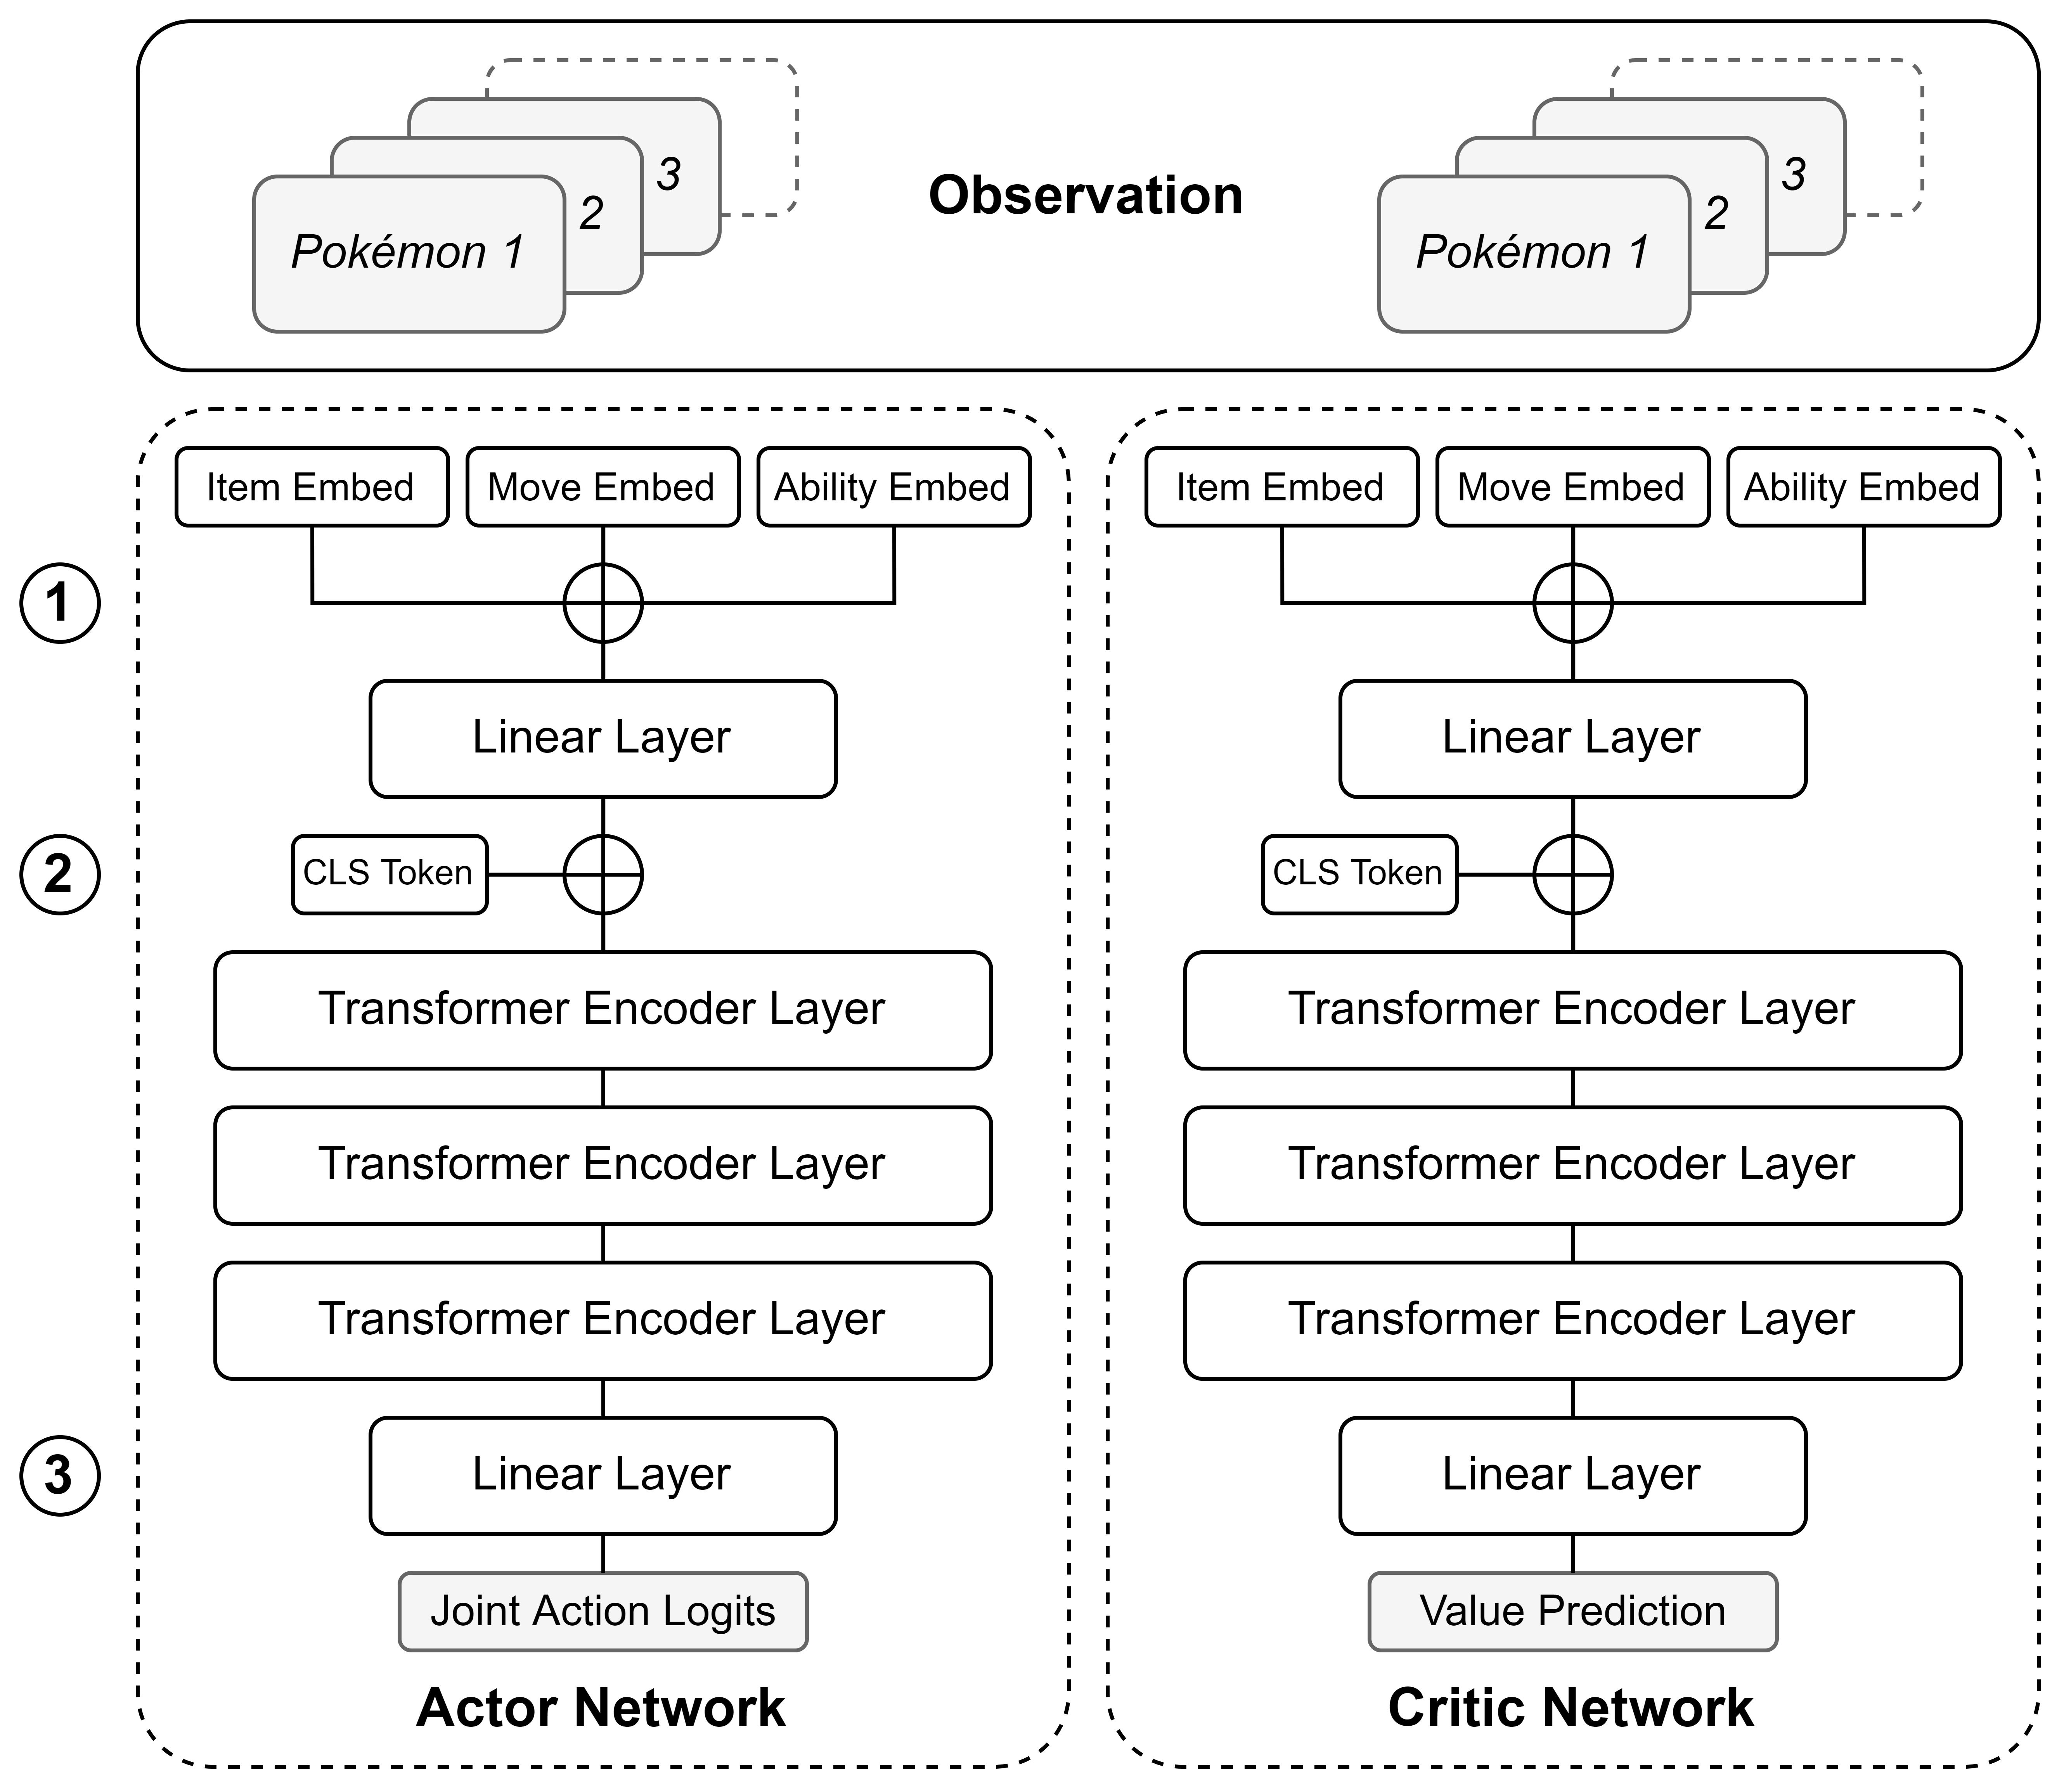
\includegraphics[width=0.95\textwidth]{images/figures/vgc-bench.png}
    \caption{The architecture used by all RL agents in VGC-Bench~\cite{angliss2025vgc}. All agents use an actor-critic framework with the same network architecture, but without direct parameter sharing. A forward pass through the network can be dissected into the following steps: \textbf{(1)} All Pokémon in the observation have their items, moves, and abilities embedded into 32-dimensional latent representations. These representations, together with other numerical features, are concatenated and projected to a single 256-dimensional latent space. \textbf{(2)} The latent vector is concatenated with an aggregation token (typically referred to as the \textit{CLS token}~\cite{devlin2019bert}), before passing through a three-layer, encoder-only transformer model with four attention heads. \textbf{(3)} The output of the transformer is either projected to action logits (actor), or to a value prediction (critic).}
    \label{fig:vgcbench-architecture}
\end{figure}

The findings of VGC-Bench show that behavior cloning fine-tuned with RL techniques can consistently beat other agents, and is even able to beat professional VGC players under the right circumstances.
They furthermore show that RL agents perform best when the amount of teams they see during training is kept to a minimum, though agents who see more teams during training are able to generalize better to unseen teams~\cite{angliss2025vgc}.
